\subsection{Hauptschleife}
    Die Hauptschleife ist der Kern des Programmes und verwaltet alle Variablen.

    \subsubsection{Zustandsmaschine}\label{Zustandsmaschine}
        Um die verschiedenen Zustände der Kerze zu verwalten, wird eine 
        Zustandsmaschine verwendet. Diese beinhaltet folgende Zustände,
        wobei die Kerze im \textit{LED\_OFF} Zustand startet.
        Bei jedem Zustandswechsel wird das \texttt{lock} Flag aktiviert und
        blockiert solange die Zustandsmaschine bis die Kerze ihre
        Ausgangsposition wieder eingenommen hat. Somit wird verhindert,
        dass eine Bewegung der Kerze mehrere Zustände überspringt.
        Die eigentliche Zustandsmaschine besteht aus dem \texttt{State} Enum
        sowie der \textit{Switch-Anweisung} in der Hauptschleife.

        \begin{figure}[H]
            \centering
            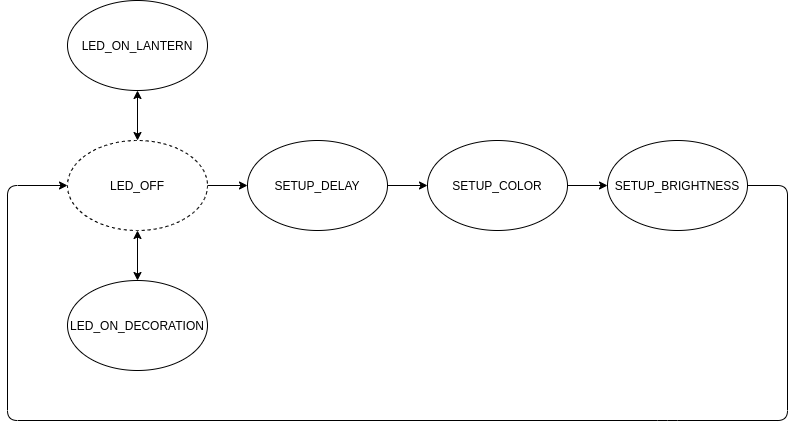
\includegraphics[scale=0.5]{img/state.png}
            \caption{Zustandsmaschine}
        \end{figure}
    
    \subsubsection{Konfiguration}
        In jedem \textit{Setup} Zustand kann das entsprechende Array
        (Siehe \ref{Datenstrukturen}) durchlaufen werden und somit die
        vordefinierten Werte in der \texttt{Config} Datenstruktur gespeichert
        werden. Der einsatz eines Arrays spart in diesem Fall mehrere Zustände,
        da nicht für jeden vordefinierten Wert ein neuer Zustand erstellt werden
        muss. Der Nachteil dieser Lösung ist der höhere Ramverbrauch durch die
        Arrays, welcher jedoch bei einer Arraygröße von drei unerheblich ist.
        Beispielhaft für dieses Verfahren wird der \textit{SETUP\_COLOR} Zustand
        beschrieben.
        \lstinputlisting[caption=SETUP\_COLOR Zustand,firstline=246, lastline=267]{../main.c}
        Die \texttt{setup\_index} Variable wird bei jedem Zustandswechsel auf
        \texttt{SETUP\_DEFAULT\_INDEX}, welches eins ist, gesetzt. Somit
        startet jeder \textit{Setup} Zustand in der Mitte des Arrays und
        ermöglicht es, durch inkrementieren von \texttt{setup\_index} einen
        höheren Wert, sowie durch das dekrementieren der Variable einen
        niedrigeren Wert zu wählen. Dabei muss zusätzlich darauf geachtet werden,
        dass es zu keinem Über- bzw. Unterlauf kommt.


